\documentclass[11pt,spanish,answers]{exam}
\usepackage[utf8]{inputenc}
\usepackage[absolute]{textpos}
\usepackage{physics}
\usepackage{stackengine}
\usepackage{tikz}
\usetikzlibrary{chains,positioning,decorations.pathreplacing,arrows}



\usepackage{babel}
\usepackage{amsmath}
\title{Tarea I: Calentamiento}
\author{Georvic Tur - 12-11402}
\date{25/04/2017}

\begin{document}

\begin{textblock}{10}(5.6,1)
    \noindent\LARGE Universidad Simón Bolívar
\end{textblock}

\begin{textblock}{10}(4.7,1.5)
    \noindent\LARGE Departamento de Cómputo Científico
\end{textblock}

\maketitle

\renewcommand{\solutiontitle}{\noindent\textbf{Solución:}\par\noindent}

\begin{questions}

\question
La función logística se define como 
\begin{equation} \label{eq1}
    \begin{split}
        \varphi(v) & = \frac{1}{1 + \exp(-v)}
    \end{split}
\end{equation}
con rango entre 0 y 1. Muestre que la derivada satisface la siguiente relación:
\begin{equation} \label{eq2}
    \begin{split}
        \dv{\varphi}{v} & = \varphi(v)[1-\varphi(v)]
    \end{split}
\end{equation}
¿Cuál es el valor de la derivada en el origen?

    \begin{solution}
    
        Derivemos paso por paso la función $\varphi$. Si aplicamos el teorema de la derivada de una fracción, tenemos que:
        
        \begin{align*}
           \dv{\varphi}{v} &=  \frac{- \dv{(1+exp(-v))}{v}}{(1+exp(-v))^2} \tag*{(derivada de una fracción)} \\
           &= \frac{exp(-v)}{(1+exp(-v))^2}           \tag*{(regla de la cadena)} \\
           &= (\frac{1}{1+exp(-v)})*(\frac{exp(-v)}{1+exp(-v)})           \tag*{(reordenando)} \\
           &= \varphi(v)*(\frac{exp(-v)}{1+exp(-v)})           \tag*{(Sustituyendo la ecuación 1)} \\
           &= \varphi(v)*(\frac{exp(-v)+(1-1)}{1+exp(-v)})           \tag*{(Elemento neutro de la adición)} \\
           &= \varphi(v)*(1 - \frac{1}{1+exp(-v)})           \tag*{(Simplificando)} \\
           &= \varphi(v)*(1 - \varphi(v))           \tag*{(Sustituyendo la ecuación 1)} \\
        \end{align*}
        
        Ahora calculemos $  \dv{\varphi}{v} |_{v=0} $:
        
        \begin{align*}
           \dv{\varphi}{v} |_{v=0} &=  \varphi(0)*(1 - \varphi(0))  \tag*{(derivada de la logística)} \\
           &=  \frac{1}{2}*(1 - \frac{1}{2})  \tag*{(Valor de la logística en el origen)} \\
           &=  \frac{1}{4} \\
        \end{align*}
        
        
    \end{solution}

\question 
En la pregunta anterior vimos que la derivada de la función logística $(\varphi)$ se puede expresar como función de sí misma. Encuentre un resultado similar para la función de activación de la tangente hiperbólica definida como:
\begin{equation} \label{eq3}
    \begin{split}
        \tanh(v) & = \frac{\exp(v) - \exp(-v)}{\exp(v) + \exp(-v)}
    \end{split}
\end{equation}

    \begin{solution}
        Calculemos su derivada:
        
        \begin{align*}
           \tanh(v) &=  \frac{(\exp(v) + \exp(-v))(\exp(v) + \exp(-v)) - (\exp(v) - \exp(-v))(\exp(v) - \exp(-v))}{(\exp(v) + \exp(-v))^2} \tag*{(derivada de una fracción)} \\
           &=  \frac{(\exp(v) + \exp(-v))^2 - (\exp(v) - \exp(-v))^2}{(\exp(v) + \exp(-v))^2} \tag*{(Simplificando)} \\
           &=  1 - \Big(\frac{\exp(v) - \exp(-v)}{\exp(v) + \exp(-v)}\Big)^2 \tag*{(Simplificando)} \\
           &=  1 - \tanh(v) \tag*{(Ecuación 3)} \\
        \end{align*}
        
        Ahora calculemos $  \dv{\tanh}{v} |_{v=0} $:
        
        \begin{align*}
            \dv{\tanh}{v} |_{v=0} &= 1 - \tanh(0) \tag*{(Derivada de tanh)} \\
            &= 1 \tag*{(Tangente hiperbólica es cero en el origen)} \\
        \end{align*}
        
    \end{solution}

\question
Considere un grupo de personas cuyas opiniones colectivas en un tópico de interés se define como la suma pesada de las opiniones individuales. Suponga que si en el transcurir del tiempo la opinión de un miembro del grupo tiende a (concuerda con) la opinión colectiva del grupo, la opinión de ese miembro recibe un mayor peso. Si por el contrario, la opinión de ese miembro consistentemente está en desacuerdo con la opinión  colectiva, la opinión de dicho miembro se le da menos peso. Esto tiene el efecto de producir consenso en el grupo. Discuta la analogía de esta situación con alguno de
los postulados de aprendizaje.

    \begin{solution}
        Esto es similar al postulado de Hebb parafraseado por Haykin en su libro \cite{postuladoDeHebb}:
        
        \begin{enumerate}
          \item Si dos neuronas se activan simultáneamente, la fuerza de su sinapsis se incrementa
          \item Si dos neuronas se activan de manera asíncrona, entonces la fuerza de su sinapsis disminuye
        \end{enumerate}
        
        En este caso tendríamos (Haykin, 3rd ed, p. 370)
        
        \begin{center}      

            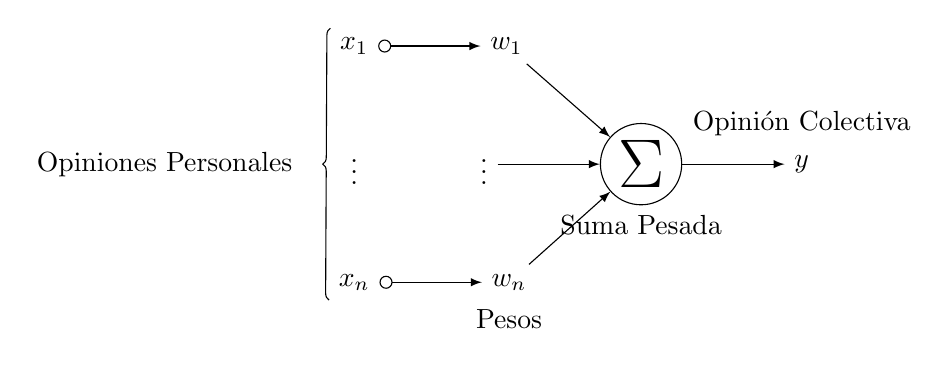
\begin{tikzpicture}[
            init/.style={
              draw,
              circle,
              inner sep=2pt,
              font=\Huge,
              join = by -latex
            },
            squa/.style={
              draw,
              inner sep=2pt,
              font=\Large,
              join = by -latex
            },
            start chain=2,node distance=13mm
            ]
            \node[on chain=2] 
              (x2) {$\vdots$};
            \node[on chain=2] 
              {$\vdots$};
            \node[on chain=2,init,label=below:Suma Pesada] (sigma) 
              {$\displaystyle\Sigma$};
            
            \node[on chain=2,label=above:Opinión Colectiva,join=by -latex] 
              {$y$};
            
            \begin{scope}[start chain=1]
            \node[on chain=1] at (0,1.5cm) 
              (x1) {$x_1$};
            \node[on chain=1,join=by o-latex] 
              (w1) {$w_1$};
            \end{scope}
            
            
            
            \begin{scope}[start chain=3]
            \node[on chain=3] at (0,-1.5cm) 
              (x3) {$x_n$};
            \node[on chain=3,label=below:Pesos,join=by o-latex] 
              (w3) {$w_n$};
            \end{scope}
            
            
            \draw[-latex] (w1) -- (sigma);
            \draw[-latex] (w3) -- (sigma);
            
            \draw[decorate,decoration={brace,mirror}] (x1.north west) -- node[left=10pt] {Opiniones Personales} (x3.south west);
            \end{tikzpicture}

        \end{center}
        
        Ese sería también uno de los principios de la auto-organización (Haykin, 3rd ed, p. 368)
        
    \end{solution}


\question
Para una red neuronal de la forma

\begin{equation} \label{eq4}
    \begin{split}
        y_k & = \sigma(\sum_{j=1}^{K} w_{kj}^{(2)} \sigma(\sum_{i=1}^{M} w_{ji}^{(1)} x_i))
    \end{split}
\end{equation}

en la cual la función de activación $\sigma$ está dada por función logística, muestre que
existe una red equivalente salvo por transformaciones lineales de los parámetros del
modelo, que calcula exactamente igual pero con función de activación  en la capa oculta
dada por la tangente hiperbólica. Ayuda: Primero encuentre una relación entre la
logística y la tangente hiperbólica.


\begin{solution}

    Supongamos que la función logística depende de tanh por las formas de sus gráficas: $\varphi(v) = a + b*\tanh(c*v + d)$. Si aplicamos límites, tenemos:
    
    \begin{align*}
        \lim_{v \to \infty} \varphi(v) &= 1 \tag*{(Límite de la logística al tender al infinito)}\\
        a + b*(\lim_{v \to \infty} \tanh(c*v+d)) &= 1 \tag*{(Sustituyendo la suposición y aplicando límite)}\\
        a + b &= 1 \tag*{(Límite de tanh al tener al infinito)}
    \end{align*}
    
    Asimismo:
    
    \begin{align*}
        \lim_{v \to -\infty} \varphi(v) &= 0 \tag*{(Límite de la logística al tender al infinito negativo)}\\
        a + b*(\lim_{v \to -\infty} \tanh(c*v+d)) &= 0 \tag*{(Sustituyendo la suposición y aplicando límite)}\\
        a - b &= 0 \tag*{(Límite de tanh al tender al infinito negativo)}
    \end{align*}
    
    Con esas dos ecuaciones tenemos $a = b = \frac{1}{2}$. Si evaluamos $\varphi(0)=\frac{1}{2}$, tenemos:
    
    \begin{align*}
        \varphi(0) &= \frac{1}{2} \tag*{(Valor de la logística)} \\
        a + b*\tanh(0 + d) &= \frac{1}{2} \tag*{(Suposición)} \\
        \frac{1}{2} + \frac{1}{2}*\tanh(0 + d) &= \frac{1}{2} \tag*{(Valores de a y b)} \\
        \tanh(d) &= 0 \tag*{(Simplificando)} \\
        &\implies \\
        d &= 0 \tag*{(Valor de tanh en el origen)} \\
    \end{align*}
    
    Si aplicamos la derivada evaluada en cero, tenemos:
    \begin{align*}
        \dv{\varphi}{v} |_{v=0} &= \frac{1}{4} \tag*{(Por la pregunta 1)} \\
        b*\Big(\dv{(\tanh(c*v+d))}{v} |_{v=0}\Big) &= \frac{1}{4} \tag*{(Por suposición y derivada de una constante)} \\
        b*c*\Big(1-tanh(c*0 + d)\Big)^2 &= \frac{1}{4} \tag*{(Por pregunta 2 y regla de la cadena)} \\
        \frac{1}{2}*c*\Big(1-tanh(0)\Big)^2 &= \frac{1}{4} \tag*{(Valores de a, b y d)} \\
        \frac{1}{2}*c &= \frac{1}{4} \tag*{(Valor de tanh en el origen)} \\
        &\implies \\
        c &= \frac{1}{2} \\
    \end{align*}
    
    Por tanto, tenemos que $\varphi(v) = \frac{1}{2} + \frac{1}{2}\tanh(\frac{1}{2}v)$. Si sustituimos a $v$ por $2v$, podemos obtener:
    
    \begin{equation} \label{eq5}
        \begin{split}
           \tanh(v) &= 2\varphi(2v) + 1
        \end{split}
    \end{equation}
    
    Con ayuda de la ecuación 5, podemos hacer lo siguiente:
    
    \begin{align*}
        y_k &= \sigma(\sum_{j=1}^{K} w_{kj}^{(2)} \tanh(\sum_{i=1}^{M} w_{ji}^{(1)} x_i)) \tag*{(Enunciado)} \\
        &= \sigma(\sum_{j=1}^{K} w_{kj}^{(2)} \Big( 2\varphi(2\sum_{i=1}^{M} w_{ji}^{(1)})+1 \Big)) \tag*{(Ecuación 5)} \\
        &= \sigma(\sum_{j=1}^{K} (2w_{kj}^{(2)}) \varphi(\sum_{i=1}^{M} (2w_{ji}^{(1)})) + \sum_{j=1}^{K} w_{kj}^{(2)}) \tag*{(Distribuyendo)} \\
    \end{align*}
    
    Donde $2w_{ji}^{(1)}$ y $2w_{kj}^{(2)}$ son transformaciones lineales de los parámetros de la red neuronal y $b = \sum_{j=1}^{K} w_{kj}^{(2)}$ puede considerarse un bias. Por tanto, hemos mostrado que una red de dos capas como la del enunciado es equivalente a otra que use en la capa oculta a $\tanh$.
    
\end{solution}

\end{questions}



\begin{thebibliography}{1}
\bibitem{postuladoDeHebb} 
Simon Haykin,
\textit{Neural networks and learning machines, 3rd ed}. 
Upper Saddle River: Pearson Education, 2009. p, 369.
\end{thebibliography}

\end{document}
